\documentclass{article}
\usepackage{geometry}
\geometry{a4paper}
\usepackage{ctex}
\usepackage{graphicx} %添加图片
\usepackage{float}
\usepackage{amsthm}
\usepackage{amsmath}
\renewcommand{\vec}[1]{\boldsymbol{#1}} % 生产粗体向量,而不是带箭头的向量
\usepackage{amssymb}
\usepackage{booktabs} % excel导出的大表格
\usepackage{hyperref}
\usepackage{listings}

\title{合成孔径雷达原理 \\ RDA成像算法实验报告}

\author{姓名:邓嘉 \\ 学号:21216293 \\ Email: \href{mailto:dengj57@mail2.sysu.edu.cn}{dengj57@mail2.sysu.edu.cn}}

\date{}

\begin{document}

\maketitle


\section{实验目的}

1. 理解RDA成像算法的原理。

2. 编写RDA算法matlab仿真程序。

3. 用仿真程序处理所给的星载数据,深入理解RDA算法的具体处理流程,并完成成像过程以及结果展示。

\section{实验原理}
\subsection{RDA算法简介}

距离多普勒算法是在1976年至1978年为处理SEASAT-SAR数据而提出的,该算法于
1978年处理出第一幅机载SAR数字图像。RDA至今仍然在广泛使用,它通过距离和方位上的频域操作,达到了高效
的模块化处理要求,同时又具有了一维操作的简便性。该算法根据距离和方位上的大尺度时间差异,在两个一维
操作之间使用距离徙动校正(RCMC),对距离和方位进行了近似的分离处理。

由于距离徙动校正是在距离时域-方位频域中实现的,所以也可以进行高效的模块化处理。因为方位向频率等同于
多普勒频率,所以该处理域又称为“距离多普勒域”。距离徙动校正的“距离多普勒”域实现是RDA与其他算法的主要
区别,因而称其为距离多普勒算法。


\subsection{RDA算法概述}
图 \ref{1} 示意了RDA的处理流程。第一种给出的是适合小斜视角及短孔径下的基本RDA处理框图。第二种方法是
斜视处理所需要的二次距离压缩改进算法,其中二次距离压缩为二维频域中的精确实现,这也是本次实验所采用
的方法。第三种是二次距离压缩的近似距离频域实现。

除了二次距离压缩实现,三种方法基本相同。

1. 当数据处在方位时域时,可通过快速卷积进行距离压缩。也就是说,进行距离快速傅里叶变换后随即进行
距离向匹配滤波,再利用距离快速傅里叶逆变换完成距离压缩。第一种和第三种就是这种情况,第二种方法则不同。

2. 通过方位向快速傅里叶变换将数据变换至距离多普勒域,多普勒中心频率估计及大部分后续操作都将在该域
进行

3. 在距离多普勒域进行随距离向时间及方位向频率变化的距离徙动校正,该域中同一距离上的一组目标轨迹相互重合。
通过距离徙动校正,将距离徙动曲线拉直到方位向频率轴平行的方向。

4. 通过每一距离门上的频域匹配滤波实现方位压缩。

5. 最后通过方位向快速傅里叶逆变换将数据变换回时域,得到压缩后的复图像,如果需要,还可以进行幅度检测
和多视叠加。(本次实验并没有实现)

\begin{figure}[H] %htbp
\centering
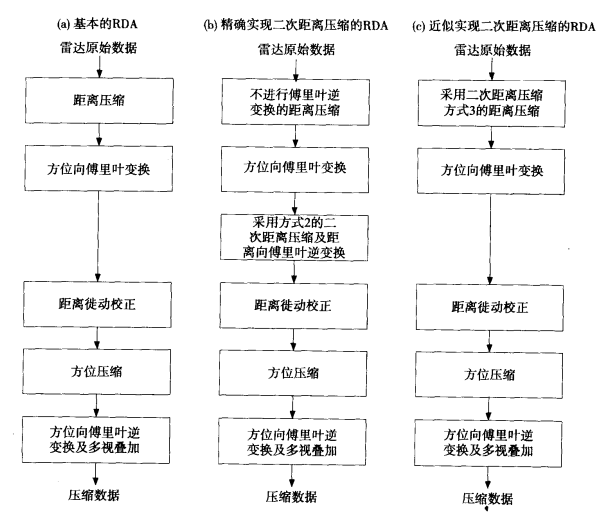
\includegraphics[scale=0.6]{1.png}
\caption{RDA的三种实现方法}
\label{1}
\end{figure}

下面对算法中的步骤细节进行分析。

(1)距离压缩

距离压缩即在距离向对信号进行脉冲压缩处理,雷达发送的是宽LFM信号,通过匹配滤波处理后,
信号变窄,提高距离向分辨率。在匹配滤波的同时,可以采用不同的窗函数抑制旁瓣,提高分辨率。
为了简便运算,RDA算法的距离压缩往往在频域进行。距离压缩输出为

\begin{equation}
	s_rc( \tau, \eta ) = IFFT_{\tau} \{ S_0(f_{ \tau}, \eta) H(f_{\tau}) \}
\end{equation}
\begin{equation}
	s_rc( \tau, \eta ) = A_0 p_r [\tau - 2\frac{R(\eta)}{c}] \omega_a (\eta - \eta_{c}) exp \{ -j4 \pi f_0 \frac{R(\eta)}{c} \}
\end{equation}

其中,压缩脉冲包络$p_r(\tau)$为窗函数$W_t(f_\tau)$的傅里叶逆变换。对于矩形窗,
$p_r(\tau)$为
$sinc$函数。对于锐化窗,$p_r(\tau)$为旁瓣较低的$sinc$函数。
式中各项因子的物理含义如下。$A_0$为包括散射系数在内的总增益,一般假定为1。
$p_r [\tau - 2\frac{R(\eta)}{c}]$为$sinc$型距离包络,其中包括了随方位变化
的目标距离徙动$2\frac{R(\eta)}{c}$。后两项给出的是与距离压缩无关的方位向上的增益和相位。


而斜距分辨率则为:
\begin{equation}
	p_r = \frac{c}{2} \frac{0.886 \gamma_{\omega,r}}{|K_r|T_r}
\end{equation}

$\gamma_{\omega,r}$为锐化窗引入的IRW展宽因子,$|K_r|T_r$为chirp带宽,引入$\frac{c}{2}$
表示分辨率量纲为长度而非时间。

(2)方位项傅里叶变换

通过方位向快速傅里叶变换,将每一距离上的数据变换到距离多普勒域。利用驻定相位原理,得到
方位向上的时频关系为

\begin{equation}
	f_\eta = -K_a \eta
\end{equation}

将$\eta = \frac{-f_\eta}{K_a}$代入,方位向快速傅里叶变换后的信号为

\begin{equation}
	S_1( \tau, f_{\eta} ) = A_0 p_r [\tau - 2\frac{R_{rd}(f_{\eta})}{c}] W_a (f_{\eta} - f{\eta_{c}}) exp \{ -j4 \pi f_0 \frac{R_0}{c} \}exp\{j \pi \frac{f_{\eta}^2}{K_a}\}
\end{equation}

上式中含有两个指数项,第一项为目标固有的相位信息,相对于诸如干涉、极化这类应用而言是
很重要的,但却与图像强度无关。第二项为具有线性调频特性的频域方位调制。

通过上述公式,我们不难得到距离多普勒域中的距离徙动为,即包络中的$R_{rd}(f_{\eta})$:

\begin{equation}
	R_{rd}(f_{\eta}) \approx R_0 + \frac{V_{r}^{2}}{2R_0}(\frac{f_\eta}{K_a})^2 = R_0 + \frac{\lambda^2R_0f_{\eta}^2}{8V_{r}^{2}}
\end{equation}

(3)距离陡动校正(RCMC)

距离徙动校正的实现方法有两种,第一种方法是在距离多普勒域中进行距离插值运算,这可以通过
基于$sinc$函数的插值处理很方便地实现。$sinc$核被锐化窗(如Kaiser窗)截断并加权。

需要校正的距离徙动为:

\begin{equation}
 	\Delta R(f_\eta)=\frac{\lambda^2R_0f_{\eta}^2}{8V_{r}^{2}}
\end{equation}

该式表明目标偏移是方位向频率$f_\eta$的函数。假设RCMC插值精确,信号变为:

\begin{equation}
	S_2( \tau, f_{\eta} ) = A_0 p_r [\tau - 2\frac{R_0}{c}] W_a (f_{\eta} - f{\eta_{c}}) exp \{ -j4 \pi f_0 \frac{R_0}{c} \}exp\{j \pi \frac{f_{\eta}^2}{K_a}\}
\end{equation}

上式中距离包络$p_r$与方位向频率无关,表明距离徙动已得到精确校正,并且能量也集中在最近斜距$\tau = 2\frac{R_0}{c}$处。

距离徙动校正插值函数的生成和使用要考虑3个因素:插值核长度、偏移量和系数值(sinc窗)。

为了快速实现插值,可以按预先定义的升采样间隔将插值函数制成表格。这样做使得不必在每个插值点
都生成sinc函数,仅需从表格中提取最近邻域的序号,提高了计算效率。

(4)方位压缩

通常,方位向处理时分辨率的可选空间较大,这是因为要达到与距离向相同的分辨率,所使用的处理
带宽一般比方位实际带宽小。利用整个带宽进行的"全分辨率"("单视")处理能使方位分辨率达到二
分之一倍天线长度的理论极限。另一方面,还可以通过低于分辨率极限的"多视"处理获得较低的图像
噪声。

进行距离徙动校正之后,即可通过匹配滤波器进行数据的方位聚焦。由于距离徙动校正后的数据
处于距离多普勒域,因而在该域中进行方位匹配滤波要方便高效得多,作为斜距$S_0$和方位向频率 
$f_\eta$的函数,匹配滤波器为:
\begin{equation}
	H_{az}(f_\eta) = exp \{ -j \pi \frac{f_{\eta}^2}{K_a} \}
\end{equation}
其中$K_a$为$R_0$的函数。

为了进行方位压缩,将距离校正之后的$S_2( \tau, f_{\eta} )$乘以频域匹配滤波器
$H_{az}(f_\eta)$,有

\begin{equation}
	S_3( \tau, f_{\eta} ) = A_0 p_r [\tau - 2\frac{R_0}{c}] W_a (f_{\eta} - f{\eta_{c}}) exp \{ -j4 \pi f_0 \frac{R_0}{c} \}
\end{equation}

再经快速傅里叶逆变换即可完成方位压缩,
\begin{equation}
	S_{ac}( \tau, \eta) = A_0 p_r [\tau - 2\frac{R_0}{c}] p_a(\eta) exp \{ -j4 \pi f_0 \frac{R_0}{c} \} exp \{ j 2\pi f_{\eta _c} \eta \}
\end{equation}


(5)二次距离压缩(SRC)

在距离多普勒域中,应使用$K_m$代替距离匹配滤波器中的初始调频率$K_r$。如果距离压缩中的
调频率为$K_r$,则需要使用一个滤波器进行插值补偿。其线性调频率$K_{src}$为:
\begin{equation}
	K_{src}(R_0,f_{\eta}) = \frac{2 V_{r}^{2} f_{0}^{3} D^3 (f_\eta,V_r)}{cR_0f_\eta ^2}
\end{equation}

也就是说,首先使用调频率为$K_r$的滤波器进行初级压缩(即标准距离压缩)
,随后使用调频率为$K_{src}$的次级滤波器进行压缩。
	
本次使用的二次距离压缩方法为方式2。此时二次距离压缩在二维频域实现,该域中需要使用固定的$R_0$
,通常取在测绘带中心。由于二次距离压缩对$R_0$的依赖较弱,所以可在全部测绘带内将其设为定值。

在方式2中,首先使用调频率为$K_r$的标准低斜视角距离匹配滤波器,此时接收脉冲中的二次相位
被完全补偿,但在信号在第二步变换到方位频域后,距离信号中出现一个较小的二次相位,若直接
进行快速傅里叶变换则会造成散焦。因此,需要通过二次距离压缩滤波器将其补偿掉。


\section{程序设计思路与代码分析}

\begin{figure}[H] %htbp
	\centering
	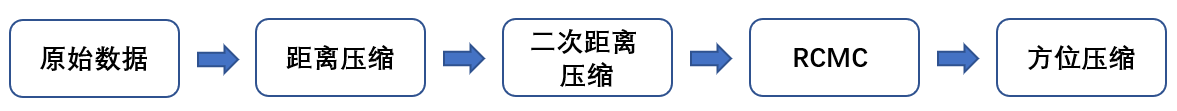
\includegraphics[scale=0.45]{2.png}
	\caption{成像流程}
	\label{2}
\end{figure}

根据实验原理部分的描述,设计的程序应该包含以下5个部分:

(1)读取数据。该部分功能为从所给数据包中提取出数据并进行保存以供后续处理。

(2)距离压缩。该部分功能为完成距离压缩,也就是在距离向上做匹配滤波。距离压缩结束后,
图像由二维时域变换到了距离频域和方位时域上。

(3)SRC。该部分功能为SRC,也就是二次距离压缩。二次距离压缩需要在二维频域上完成,因此在这一步
之前,需要完成方位向的傅里叶变换将图像从距离频域和方位时域变换到二维频域。

(4)RCMC。该部分功能为RCMC,也就是距离徙动校正。距离徙动校正需要在距离多普勒域上完成
,也就是距离时域和方位频域,因此在这一步之前需要对距离向做一次IFFT(傅里叶逆变换)。

(5)方位压缩。图像进行完RCMC后,处于距离多普勒域,此时可以直接进行方位向的频域匹配滤波,
完成方位压缩。方位压缩后再对方位向做一次IFFT(傅里叶逆变换),图像此时回到二维时域,处理
流程结束,我们可以将图像进行输出。
\begin{figure}[H] %htbp
	\centering
	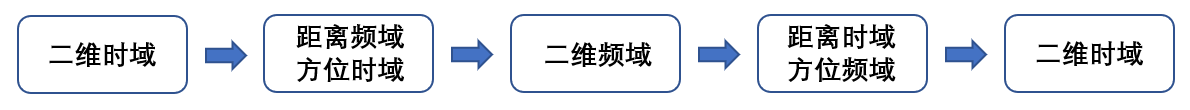
\includegraphics[scale=0.45]{3.png}
	\caption{成像过程中的域变化}
	\label{3}
\end{figure}
按照上述思路,我们开始逐一对程序各部分进行编写,代码的具体细节见注释。
\subsection{数据读取}
\begin{lstlisting}	
	%%
	%该部分的功能为提取与保存数据
	%文件初始化
	clear;
	clc;
	close all;
	load CD_run_params
	output_path = './';
	data = zeros(1536,2048);
	
	
	for b = 1 : 2
	file_pre = strcat( output_path, output_prefix, '_', num2str(b) );
	AGC_values = load_AGC_block( file_pre, first_rg_line, ...
	Nrg_lines_blk, b , UseMATfiles ); 
	data(:,:,b) = load_DATA_block( file_pre, output_path, ...
	Nrg_lines_blk, Nrg_cells, AGC_values, b, UseMATfiles );
	end
	data = double(data);
	s_echo = [data(:,:,2);data(:,:,1)];
	
	figure;
	image(abs(s_echo));
	title('原始图像/二维时域');
	colormap(gray);
	colorbar;
\end{lstlisting}
该部分结束后输出结果如下:

\begin{figure}[H] %htbp
	\centering
	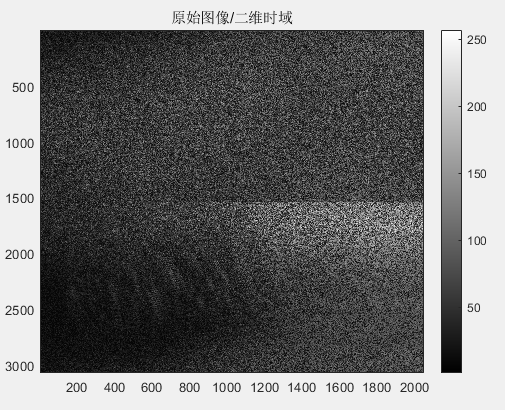
\includegraphics[scale=1]{4.png}
	\caption{原始图像/二维时域}
	\label{4}
\end{figure}

\subsection{参数定义}
\begin{lstlisting}
	%%
	%该部分的功能为定义一些参数
	%方位向:Azimuth
	%距离向:Range
	Kr = -Kr;                       % 将调频率Kr改成负值
	BW_range = 30.111e+06;          % 脉冲宽度
	Vr = 7062;                      % 有效雷达速率
	KA = 1733;                      % 方位调频率
	f_doppler = -6900;                    % 多普勒中心频率
	FA = PRF;                       % 方位向采样率
	lamda = c/f0;                   % 波长
	T_start = 6.5959e-03;           % 数据窗开始时间
	Nr = round(Tr*Fr);              % 线性调频信号采样点数
	Nrg = Nrg_cells;                % 距离线采样点数
	Naz = Nrg_lines;          % 总共的距离线数
	NFFT_rg = Nrg;            % 距离向FFT长度
	NFFT_az = Naz;           % 方位向FFT长度
	% 距离
	% 距离时间轴
	tr = T_start + ( -Nrg/2 : (Nrg/2-1) )/Fr;                       
	% 距离频率轴
	fr = ( -NFFT_rg/2 : NFFT_rg/2-1 )*( Fr/NFFT_rg );                 
	% 方位
	 % 方位时间轴
	ta = ( -Naz/2: Naz/2-1 )/FA; 
	% 方位频率轴
	fa = f_doppler + ...
	fftshift(-NFFT_az/2:NFFT_az/2-1)/NFFT_az*FA; 
\end{lstlisting}




\subsection{距离压缩}
\begin{lstlisting}
	%%  
	% 距离压缩
	% 首先先进行距离向上的傅里叶变换
	S_range = fft(s_echo,NFFT_rg,2);  
	% 生成距离向匹配滤波器,采用方式2
	% 时域复制脉冲,末端补零后进行FFT,最后取复共轭
	t_ref = ( -Nr/2 : (Nr/2-1) )/Fr;    % 用来生成距离时间轴
	t_ref_mtx = ones(Naz,1)*t_ref;      % 矩阵形式
	w_ref = kaiser(Nr,2.5);             % 距离向,构建Kaiser窗
	w_ref = ones(Naz,1)*(w_ref.');      
	% 构成矩阵形式,每一行都进行加窗操作
	
	s_ref = w_ref.*exp((1j*pi*Kr).*((t_ref_mtx).^2)); 
	%加了窗的复制(发射)脉冲。
	s_ref = [s_ref,zeros(Naz,Nrg-Nr)];     
	% 对复制脉冲,后端补零。
	 
	S_ref = fft(s_ref,NFFT_rg,2);         
	% 复制脉冲的距离傅里叶变换。
	H_range = conj(S_ref);                 % 距离向匹配滤波器。
	S_range_c = S_range.*H_range;  % 乘以匹配滤波器。          
	% 为了作比较,先变换回二维时域
	s_rc = ifft(S_range_c,[],2);   
	
	% 作图显示
	figure;
	imagesc(abs(s_rc));
	title('距离压缩后/二维时域'); 
	colormap(gray);
	colorbar;
\end{lstlisting}
运行结果如下:

\begin{figure}[H] %htbp
	\centering
	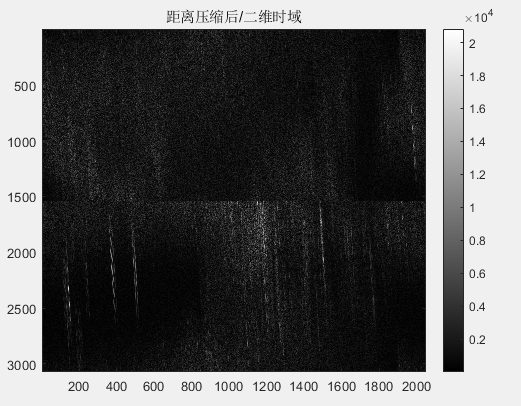
\includegraphics[scale=1]{5.png}
	\caption{完成距离压缩/二维时域}
	\label{5}
\end{figure}




\subsection{二次距离压缩(SRC)}
\begin{lstlisting}
	%%
	% 该部分完成的功能为二次距离压缩(SRC)
	% 距离压缩需要在频域完成
	% 在二维时域进行数据搬移
	s_rc = s_rc.*exp(-1j*2*pi*f_doppler.*(ta.'*ones(1,Nrg))); 
	% 方位向傅里叶变换,到距离多普勒域
	S_2df = fft(s_rc,NFFT_az,1);
	% 距离向傅里叶变换,到二维频域
	S_2df = fft(S_2df,Nrg,2);               
	
	% 大斜视角下的徙动因子
	D_fn_Vr = sqrt(1-lamda^2.*(fa.').^2./(4*Vr^2));         
	K_src = 2*Vr^2*f0^3.*D_fn_Vr.^3./(c*R0*(fa.').^2);   
	K_src_1 = 1./K_src;
	% 二次距离压缩滤波器
	H_src = exp(-1j*pi.*K_src_1*(fr.^2)); 
	H_src = fftshift(H_src,2);   
	
	S_2df_src = S_2df.*H_src;  
	% 完成二次距离压缩(SRC),回到距离多普勒域。
	S_rd = ifft(S_2df_src,[],2);  
	
	
	% 作图显示
	figure;
	imagesc(abs(S_rd));
	title('SRC后/距离多普勒域');
	colormap(gray);
	colorbar
\end{lstlisting}
运行结果如下:

\begin{figure}[H] %htbp
	\centering
	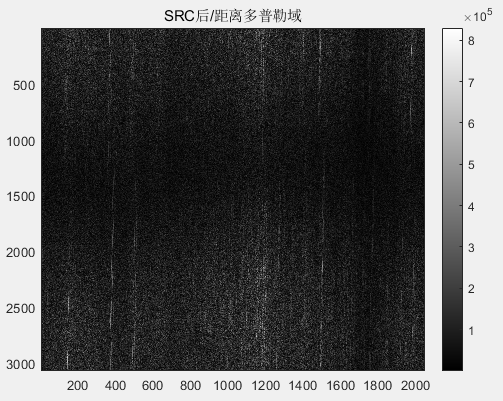
\includegraphics[scale=1]{6.png}
	\caption{SRC后/距离多普勒域}
	\label{6}
\end{figure}




\subsection{距离徙动校正(RCMC)}
该部分代码量较大,就不放到文档里了,这里说一下代码编写的具体思想。

首先这一部分代码应该完成的功能为距离徙动校正,也即RCMC,距离徙动校正应该在距离多普勒域完成,
而在上一部分代码结束时,也就是完成二次距离压缩(SRC)后,我们已经将数据从二维频域搬移到距离多普勒域上,
因此这里可以直接进行数据的操作,而不需要进行域的变化。

其次我们选择的插值核长度为8,这主要是基于计算量和精度的选择。同时由于数据只有整数点取值,且范围有限。
因此在插值中必须要考虑它的取值溢出边界问题,代码中采取了循环移位的思想,用来解决取值溢出问题。

\begin{figure}[H] %htbp
	\centering
	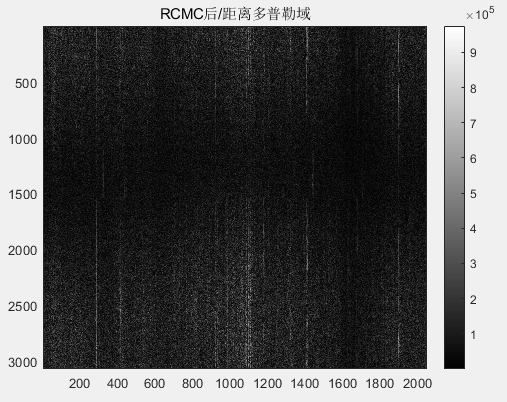
\includegraphics[scale=1]{7.png}
	\caption{RCMC后/距离多普勒域}
	\label{7}
\end{figure}

\subsection{方位压缩}
方位压缩实际上就是在方位向上做匹配滤波,非常的简单。
\begin{lstlisting}
	%%
	%该部分完成的功能为方位压缩
	fa_azimuth_MF = fa;         
	% 方位频率轴,采用和RCMC中所用的频率轴相同。
	Haz = exp(1j*4*pi.*(D_fn_Vr*R0_RCMC).*f0./c);   
	% 改进的方位向MF
	
	S_rd_c = S_rd_rcmc.*Haz;            
	% 乘以匹配滤波器
	s_ac = ifft(S_rd_c,[],1);       	
	% 完成方位压缩,变到图像域。结束。
	
\end{lstlisting}


\begin{figure}[H] %htbp
	\centering
	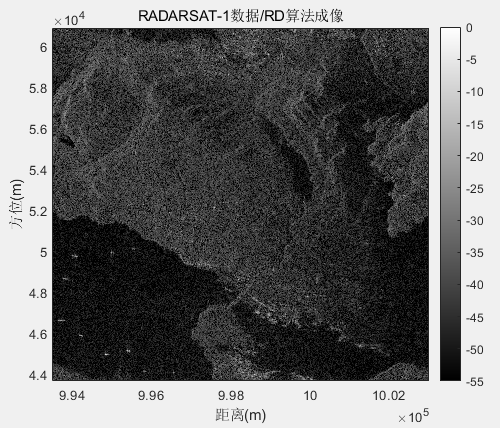
\includegraphics[scale=1]{8.png}
	\caption{RDA算法成像结果}
	\label{8}
\end{figure}

\section{实验结果与展示}
如图 \ref{9} 所示,在specify\_parameters.m文件中修改参数,
对不同地点进行成像展示。

\begin{figure}[H] %htbp
	\centering
	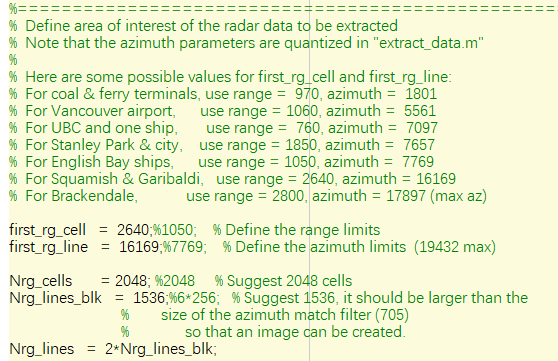
\includegraphics[scale=0.6]{9.png}
	\caption{specify\_parameters.m}
	\label{9}
\end{figure}



\subsection{coal \& ferry terminals}
\begin{figure}[H] %htbp
	\centering
	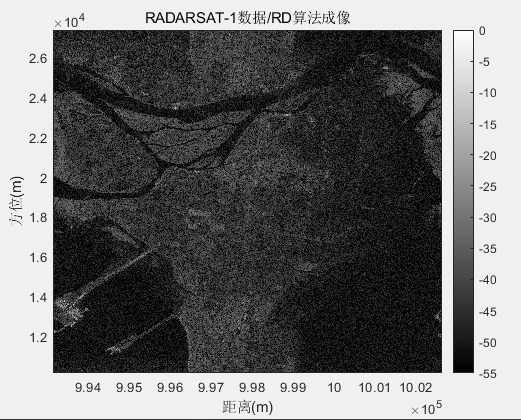
\includegraphics[scale=0.6]{10.png}
	\caption{coal \& ferry terminals}
	\label{10}
\end{figure}



\subsection{Vancouver airport}
\begin{figure}[H] %htbp
	\centering
	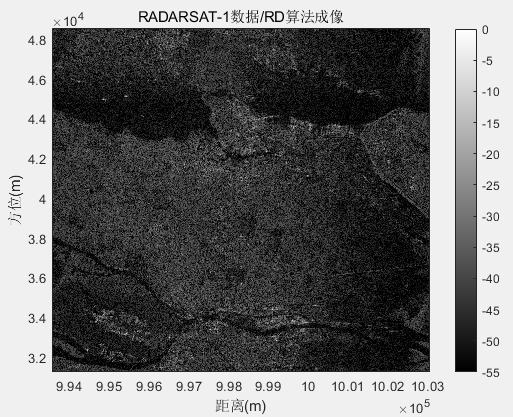
\includegraphics[scale=0.6]{11.png}
	\caption{Vancouver airport}
	\label{11}
\end{figure}

\subsection{Stanley Park \& city}
\begin{figure}[H] %htbp
	\centering
	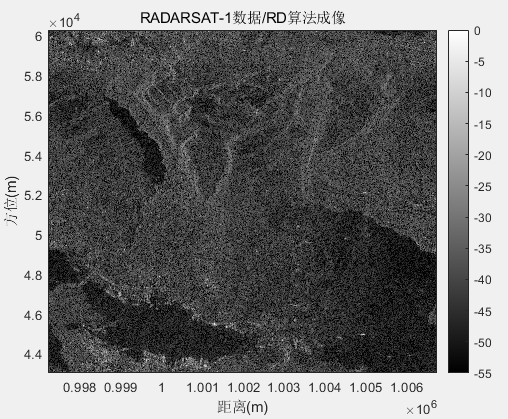
\includegraphics[scale=0.6]{12.png}
	\caption{Stanley Park \& city}
	\label{12}
\end{figure}

\subsection{Squamish \& Garibaldi}
\begin{figure}[H] %htbp
	\centering
	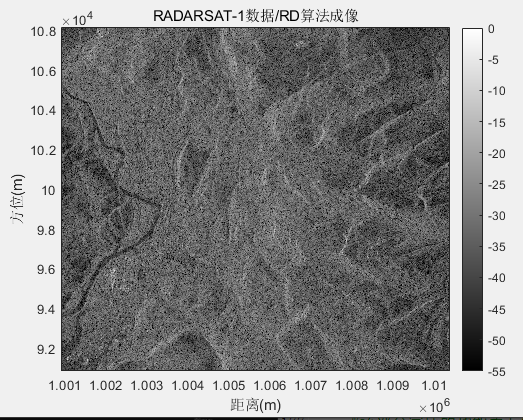
\includegraphics[scale=0.6]{13.png}
	\caption{Squamish \& Garibaldi}
	\label{13}
\end{figure}


\end{document}